% !TeX document-id = {b5392a94-51a3-49d1-9ba5-698bc09f9d35}
% !TeX encoding = UTF-8
% !TeX spellcheck = en_US
% !TeX TXS-program:bibliography = biber -l zh__pinyin --output-safechars %

\documentclass[a4paper,11pt]{article}

\newcommand{\hwNumber}{Final}

% Templates: 82ccb576e4df24e5eac4194b76230be360b4f733

% to be `\input` in subfolders,
% ... therefore the path should be relative to subfolders.

\usepackage[UTF8
	,heading=false
	,scheme=plain % English Document
]{ctex}
\usepackage{indentfirst}

\input{../.modules/basics/macros.tex}
\input{../.modules/preamble_base.tex}
\input{../.modules/preamble_notes.tex}

\newcommand{\legacyReference}{{
%	\clearpage\par
%	\quad\clearpage
	\renewcommand{\midquote}{\textbf{PAST WORK, AS TEMPLATE}}
	\newparagraph
}}

% Settings
\counterwithout{equation}{section}
\mathtoolsset{showonlyrefs=false}
%\DeclareTextFontCommand{\textbf}{\sffamily}
\renewcommand{\midquote}{\quad}

% Spacing
\geometry{footnotesep=2\baselineskip} % pre footnote split
\setlength{\parskip}{.5\baselineskip}
\renewcommand{\baselinestretch}{1.15}

%Title
	\posttitle{
		\hfill\Large\ccbyncsajp
		\par\end{flushleft}%
		\vspace*{-.7ex}\hrule%
	}
	\preauthor{\vspace{-1.5ex}%
		\flushleft\itshape%
	}
	\postauthor{\hfill}
	\predate{\noindent\ttfamily Compiled @ }
	\postdate{\vspace{.5ex}}

	\title{Advanced QFT \textnumero\hwNumber}
	\author{\signature Bryan}
	\date{\today}

% List
	\setlist*{
		listparindent=\parindent
		,labelindent=\parindent
		,parsep=\parskip
		,itemsep=1.2\parskip
	}

\input{../.modules/basics/biblatex.tex}

\title{The Geometry of Gauge Fields}
\addbibresource{gauge.bib}

%%% ID: sensitive, do NOT publish!
\InputIfFileExists{../id.tex}{}{}
\usepackage{cancel}

\begin{document}
\maketitle
\pagestyle{headings}
\pagenumbering{arabic}
\thispagestyle{empty}

%\vspace*{-1.5\baselineskip}

\setlength{\parskip}{.1\baselineskip}
\tableofcontents
\setlength{\parskip}{\parskipnorm}

\section{Introduction}
	A common way to introduce gauge fields in a non-gauge system is by promoting some global symmetry to a local one. For example, consider some fundamental matter with $\mrm{SU}(N)$ global symmetry, and we have: 
	\begin{equation}
		\mcal{L}
		= -\bar{\psi} \gamma^\mu \pdd{\mu} \psi
		\quad\longmapsto\quad
			-\bar{\psi} \gamma^\mu D_\mu \psi,
		\quad
			D_\mu = \pdd{\mu} + A_\mu
	\end{equation}
	The $\mrm{SU}(N)$ gauge potential $A_\mu$ arises naturally as a \textit{connection}, and $D_\mu$ serves as the \textit{covariant derivative}, such that the Lagrangian is manifestly invariant under the local $\mrm{SU}(N)$ symmetry. This is very much similar to the geometry of general relativity; in fact, the notion of \textit{curvature} as a geometric invariant generalizes nicely in this framework, leading to the definition of the gauge-invariant field strength:
	\begin{equation}
		F_{\mu\nu} = [D_\mu,D_\nu]
	\end{equation}
	
	However, such na\"ive analogy between gauge theory and relativity has its limitation, since gravity itself is only a very special example of gauge theory. In general, the matter fields in a gauge theory may live on some non-trivial fiber over the base manifold, while in gravity the basic fiber is simply the tangent space of the base manifold. Therefore, for a generic gauge theory, it is helpful to look at the more general mathematical structure — a \textit{vector bundle}, to better understand the geometry of gauge theory. 
	
	This note aims to provide a minimal introduction to the basic pictures of vector bundles and its applications in gauge theory. We will try to capture the basic concepts  in a less rigorous manner, without getting lost in the realm of definitions. Our main references are \textit{Baez \& Muniain} \cite{baez1994gauge}, \textit{Marsh} \cite{Marsh:2016hdj}, \textit{Göckeler \& Schücker} \cite{gockeler1989differential} and \textit{Nakahara} \cite{Nakahara:2003nw}. 
\section{Basics of Bundles}
\subsection{Vector Bundle}
	A \textit{fiber bundle} $E$ is a ``bundle'' of identical fibers $\{E_p \,|\, E_p\cong F\}_{p\in M}$ with smooth projections down to the base manifold $\pi\colon E\to M$. When the fiber is a vector space, it is then a vector bundle. 
	
	\begin{figure}[!ht]
	\centering
	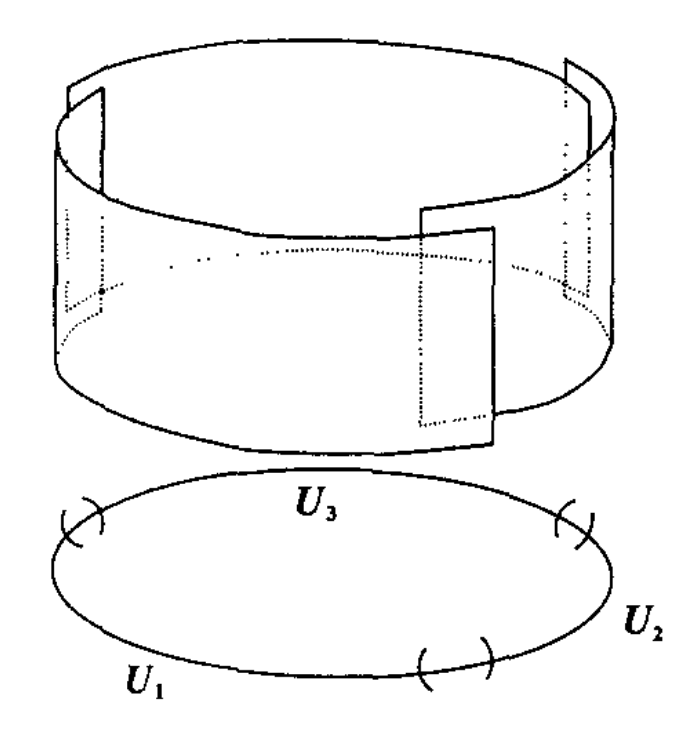
\includegraphics[width=.3\linewidth]{img/bundle_construct.png}
	\caption{Building a bundle out of trivial bundles; image borrowed from \cite{baez1994gauge}. }
	\label{fig:bundle_construct}
	\end{figure}
	
	As is common in differential geometry, such object can be constructed by gluing some trivial parts together; in this case it is some simple product spaces $\{U \times F \,|\, U \subset E\}$ with overlaps, as is shown in \autoref{fig:bundle_construct}. This is the \textsc{vector bundle construction theorem}. However, we have to make sure that such gluing is compatible between patches, without producing some nasty singularities. This can be achieved by imposing consistency conditions on \textit{transition functions} \cite{baez1994gauge,Nakahara:2003nw} between patches. 
	
	More specifically, consider the \textit{local trivialization} $\Phi\colon \pi^{-1}(U)\to U\times F$ that realizes the identification of some region $\pi^{-1}(U)\in E$ to the product space $U \times F$. This, in effect, specifies a coordinate patch on $\pi^{-1}(U)$. Coordinate transformations between patches are then given by the transition function:
	\begin{equation}
		\Phi_U\circ\Phi_V^{\smash{-1}}
			\big|_p
		= g_{UV} (p),\quad
		g_{UV}
		\in \mrm{GL}(n,\mbb{C})
		= \mop{End} F
	\end{equation}
	For a tangent bundle, $g_{UV}$ is precisely the \textit{Jacobian matrix} between different coordinates. Here $\mquote{g}$ stands for \textit{gauge}, not to be confused with the metric tensor. 
	
	Note that transition functions form a representation of some group $G$ on the fiber $F$:
	\begin{equation}
		g_{UV}(p)
		\in G \subset \mop{End} F
	\end{equation}
	The compatibility between patches is further ensured by the \textit{cocycle condition}: $
		g_{UV}
		\circ g_{VW}
		\circ g_{WU} = \idty
	$. Sometimes it is possible to restrict the type of transitions between patches to a subgroup of $\mrm{GL}(n,\mbb{C})$, which leads to additional structure of the vector bundle; for example, restriction to $G = \mrm{O}(3)$ means that there is a consistently defined \textit{metric} on the bundle. 
	
	In the mathematics literature, $G$ is commonly referred to as the \textit{structure group} \cite{lee2012introduction}; however, in a physicist's point of view, this is precisely the \textit{gauge group} \cite{baez1994gauge}. Gauge transformations are then reduced to coordinate transformations on the bundle, which are different descriptions of the same geometry. This is in agreement with physics, where different gauges are only different descriptions, leading to the same physical result. 
\subsection{Principal Bundle}
	In general, it is possible to remove all unnecessary data of a vector bundle, leaving only the information of how it transitions between patches. This gives the so-called \textit{principal bundle}. Intuitively, we can extract a principal bundle $P$ from a vector bundle, by replacing each of its fiber with the gauge group $G$ itself. Then the transition between patches is simply a usual group multiplication on $G$. 
	
	All gauge transformations are then encoded in the transitions between local sections of the principal bundle. It is then straight-forward to reconstruct the \textit{associated vector bundle} from the principal bundle, where the fiber $F$ serves as a point-wise representation of the gauge group $G$. Different choices of the $G$-representation $F$ corresponds to different types of matter $\psi$, which gets coupled to the gauge potential. 
	
	In fact, the connection on the associated vector bundle can be induced from the connection on the principal bundle, as we shall see below. 
\section{Connection and its Applications}
\subsection{Connection on the Vector Bundle}
	To introduce a connection on the vector bundle, consider a set of frame fields $\{e_i\}_{i = 1}^n$ which spans $F$ at each point $p$. For a trivial bundle $M\times F$ with a parallel-transported $\{e_i\}$, we would expect $D_\mu e_i = 0$; however, for a non-trivial bundle, or even a trivial bundle with non-parallel $\{e_i\}$, we should expect ``twists'' on the ``vertical'' fiber direction. 
	
	For example, consider the world-volume of the comoving frame $\{e_i\}$ of a spinning top; it forms a trivial vector bundle based on the worldline $\mbb{R}$, however $D_\mu e_i \ne 0$ due to the non-trivial spinning $\{e_i\}$. Such ``twists'' would lead to a non-trivial connection:
	\begin{equation}
		D_\mu e_j
		= A^i_{\mu j} e_i
		= A^a_\mu\,\pqty{T_a}\id{^i_j} e_i,
	\quad
		A^i_{\mu j}
		= A^a_\mu\,\pqty{T_a}\id{^i_j}
	\end{equation}
	A visualization of the fiber structure is shown in \autoref{fig:vertical_derivative}. 
	This is very much similar to basic differential geometry, where we have $e_\mu = \pd_\mu$ in place of $e_i$, and $A^i_{\mu j}$ becomes the Levi-Civita connection $\Gamma^\lambda_{\mu\nu}$. 
	
	\begin{figure}[!ht]
	\centering
	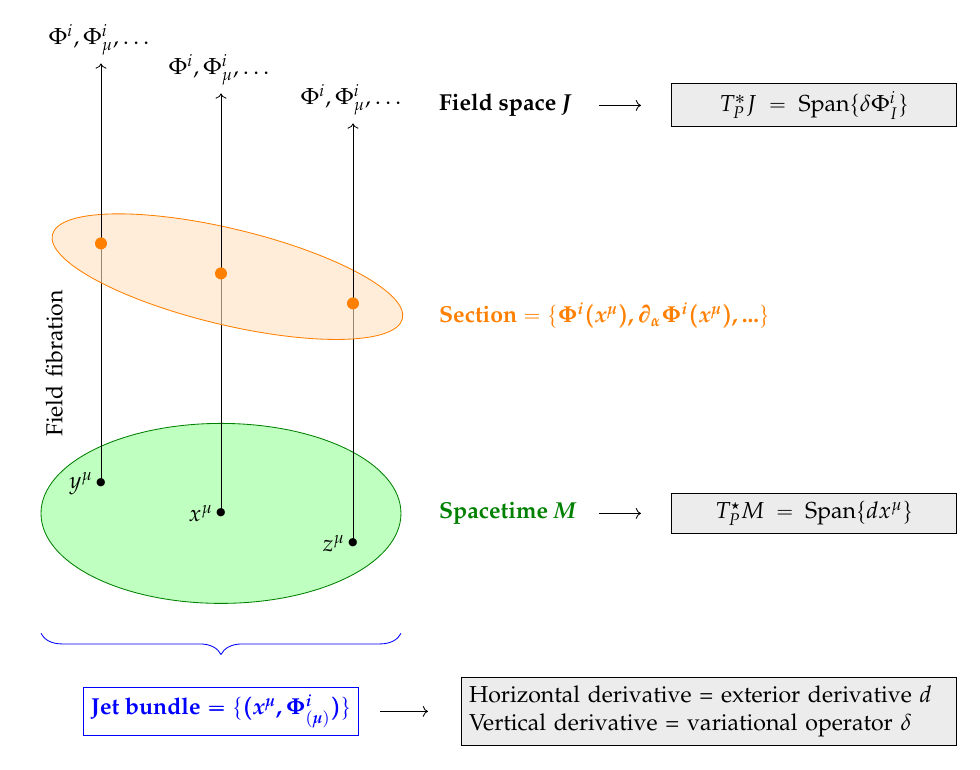
\includegraphics[width=.85\linewidth]{img/vertical_derivative.png}
	\caption{Illustration of a fiber bundle, with vertical field space and horizontal spacetime. This image also shows some additional structure: if we include ``descendants'' fields such as $
		\pdd{\mu}\psi,\,\pdd{\mu}\pdd{\nu}\psi,\cdots
	$ in the fiber, then we have a \textit{jet bundle}, which is useful in the study of Noether's theorem and conserved charges. This image is borrowed from \cite{Compere:2018aar}. }
	\label{fig:vertical_derivative}
	\end{figure}
	
	The ability to split $
		A^i_{\mu j}
		= A^a_\mu\,\pqty{T_a}\id{^i_j}
	$ relies on our discussion from the last section: there is only one true connection given the gauge structure of the vector bundle, and that is the connection on the principal bundle. All other connections are then induced from the connection on the principal bundle, labeled by the representation $\pqty{T_a}\id{^i_j}$. It is then convenient to write $A_\mu = A^a_\mu\,T_a$, with the $i,j,\cdots$ indices suppressed. Alternatively, since $T_a$ belongs to the Lie algebra $\mfrak{g} = \mop{Lie} G$, we can think of $A_\mu$ as a $\mfrak{g}$-valued function. 
	
	We can then derive the gauge transformation of $A_\mu$, by comparing with the usual Levi-Civita connection. Recall that under a coordinate transformation $x^\mu \to x'^{\mu'}$, we have:
	\begin{equation}
	\begin{aligned}
		{\Gamma'}^{\lambda'}_{\mu'\nu'}
		&= \dd{x'^{\lambda'}}
			\nabla'_{\mu'}
			e'_{\nu'},
		\quad
			e'_{\nu'}
			= \pdv{x'^{\nu'}}
			= \pdv{x^\nu} \pdv{x^\nu}{x'^{\nu'}}
			= e_\nu \pdv{x^\nu}{x'^{\nu'}},
		\\[.5ex]
		&= \pdv{x'^{\lambda'}}{x^\lambda}\,
			\Gamma^{\lambda}_{\mu\nu}\,
			\pdv{x^\mu}{x'^{\mu'}}
			\pdv{x^\nu}{x'^{\nu'}}
			+ \dd{x'^{\lambda'}} e_\nu\,
				\pdv{x'^{\mu'}}
				\pdv{x^\nu}{x'^{\nu'}}
		\\[.5ex]
		&= \pqty\bigg{\pdv{x'^{\lambda'}}{x^\lambda}}\,
			\Gamma^{\lambda}_{\mu\nu}\,
			\pdv{x^\mu}{x'^{\mu'}}
			\pqty{\pdv{x^\nu}{x'^{\nu'}}}
			+ \pqty\bigg{\pdv{x'^{\lambda'}}{x^\lambda}}\,
				\delta^\lambda_\nu\,
				\pdv{x'^{\mu'}}
				\pqty{\pdv{x^\nu}{x'^{\nu'}}}
	\end{aligned}
	\end{equation}
	We can repeat the same process but with a gauge transition Jacobian $g\id{^{i'}_{i}}$ in place of $
		\pdv{x'^{\lambda'}}{x^\lambda}
	$, while keeping the $\mu$ index fixed; this gives:
	\begin{equation}
		A'_\mu
		= g A_\mu g^{-1}
			+ g\,\pdd{\mu} (g^{-1})
	\end{equation}
	Consider the abelian case where $g = e^{-\lambda(x)}$, then this reduces to the usual electromagnetic gauge transformation: $A' = A + \dd{\lambda}$. It is then easy to verify the gauge covariance of $D_\mu$:
	\begin{equation}
		D'_\mu
		= \pdd{\mu}
			+ g A_\mu g^{-1}
			+ g\,\pdd{\mu} (g^{-1})
		= g\circ D_\mu \circ g^{-1}
	\end{equation}
\subsection{Holonomy}
	With the notion of connection, it is then possible to discuss \textit{parallel transport} in a more precise language. In fact, parallel transport of $\psi = \psi(t)$ along a curve $\gamma(t)$ is given by the familiar equation:
	\begin{gather}
		\pqty{\gamma'(t)}^\mu D_\mu \psi(t)
		= \pqty{
				\dv{t} + A\pqty{\gamma'(t)}\!
			}\,\psi(t)
		= 0,\\
		A\pqty{\gamma'(t)}
		= A_\mu \dd{x^\mu}
			\pqty{\gamma'^\nu \pdd{\nu}}
		= \gamma'^\mu A_\mu,
	\end{gather}
	This first order differential equation can be solved perturbatively, just as we did for the Schr\"odinger equation. Instead of time ordering, the result is written formally as the \textit{path-ordered exponential}:
	\begin{equation}
		H_\gamma = \mcal{P} \exp \Bqty{
				- \int_0^t A\pqty{\gamma'(t)} \dd{t}
			}
		= \mcal{P} e^{-\int_\gamma A},
		\quad
			\psi(t) = H_\gamma \psi(0)
	\end{equation}
	
	This is the expression that we acquired when studying Dirac's monopole \cite{Sakurai:2011zz}: if the gauge group $G$ is abelian, then the path ordering has no effect, and we have:
	\begin{equation}
		\psi(t)
		= e^{-\int_\gamma A} \psi(0),
		\quad
			A = A_\mu \dd{x^\mu}
	\end{equation}
	which describes the phase acquired by a charged particle as it moves along a path through a magnetic field. To restore the usual convention in electromagnetism, we should replace $A\mapsto ieA$, and we can see that it is indeed the familiar phase factor. 
	
	$H_\gamma$ as a linear map from $E_0$ to $E_p$ is called the \textit{holonomy} along the path $\gamma$. By applying gauge transformation to the parallel transport equation, we can verify that $H_\gamma$ transforms nicely under $g$:
	\begin{equation}
		H_\gamma(D')
		= g_t H_\gamma(D)\, g^{-1}_0,
		\quad
			g_t = g(p)|_{p = \gamma(t)},
		\quad
			D' = \pd + A'
	\end{equation}
	But for non-abelian $G$, $H_\gamma$ is not exactly gauge invariant. However, if $\gamma$ is a loop: $\gamma(T) = \gamma(0)$, then $\Tr H_\gamma$ is gauge-invariant. This gives the famous \textit{Wilson loop}:
	\begin{equation}
		W_\gamma
		= \Tr H_\gamma
		= \Tr \mcal{P} e^{-\int_\gamma A}
	\end{equation}
	
	Finally, recall that in differential geometry, curvature is basically holonomy along a small loop; more specifically, we have:
	\begin{equation}
		H_\gamma
		= 1 - \epsilon^2 F_{\mu\nu}
	\end{equation}
	Where $\gamma$ is a small square in the $x^\mu$--$x^\nu$ plane with a size of $\epsilon^2$. The proof of this in the context of vector bundles is identical to that in differential geometry, see e.g.~\cite{carroll_2019}. In fact, it is natural to motivate the abstract definition of curvature using this relation. 
\subsection{Curvature}
	As is mentioned before, it is straight-forward to generalize the Riemannian curvature on a vector bundle; we have:
	\begin{equation}
		F(u,v)
		\equiv [D_u\,,D_v] - D_{[u,v]},
	\end{equation}
	It is illuminating to rewrite this in terms of differential forms:
	\begin{gather}
		\pqty{F_{\mu\nu}}\id{^i_j}
		= e^i \,\pqty{2 D_{[\mu} D_{\nu]}}\, e_j,
	\\[.5ex]
	\begin{aligned}
		e^i D_\mu D_\nu e_j
		&= D_\mu \pqty{e^i D_\nu e_j}
			- (D_\mu e^i)(D_\nu e_j) \\
		&= \pdd{\mu} A^i_{\nu j}
			- (-A^i_{\mu k} e^k)
				(A^\ell_{\nu j} e_\ell) \\
		&= \pdd{\mu} A^i_{\nu j}
			+ A^i_{\mu k} A^k_{\nu j},
	\end{aligned}
	\\
		F
		= \frac{1}{2}\,F_{\mu\nu}
			\dd{x^\mu} \wedge \dd{x^\nu}
		= \pqty\Big{
				\pdd{[\mu} A_{\nu]}
				+ A_{[\mu} A_{\nu]}
			} \dd{x^\mu} \wedge \dd{x^\nu}
		= \dd{A} + A\wedge A
	\end{gather}
	
	In fact, this result is none other than \textit{Cartan's (second) structural equation} in differential geometry \cite{gockeler1989differential,liangcanbin2006relativity}. It is more commonly written as $
		\Omega
		= \dd{\omega} + \omega\wedge\omega
	$ in mathematics literature. Again, if we have $e_i\mapsto e_\lambda = \pd_\lambda$, we recover the Riemann curvature $
		\pqty{F_{\mu\nu}}\id{^i_j}
		\mapsto R\id{^\lambda_{\sigma\mu\nu}}
	$. 
	
	The Lagrangian is then constructed from the gauge-invariant, local field strength. This is when we see the difference between gravity and a generic, Yang--Mills theory. In gravity, all 4 indices of the field strength are spacetime indices, therefore we can construct a scalar curvature by tracing over indices: 
	\begin{equation}
		\mcal{L}
		\quad\sim\quad
			R
			= R\id{^\sigma_\sigma}
			= g^{\sigma\nu} R\id{^\mu_{\sigma\mu\nu}}
		\pagebreak
	\end{equation}
	Note that the metric $g_{\mu\nu}$ itself is also a dynamic field in gravity, resulting in a non-trivial base manifold $M$. On the other hand, in a generic Yang--Mills theory, it is impossible to construct a $\order{F}$ Lagrangian, since we only have 2 anti-symmetric spacetime indices, and 2 fiber indices. The only choices are then of $\order{F^2}$, for example,
	\begin{equation}
		\mcal{L}
		\quad\sim\quad
			\Tr \pqty{F\wedge\star F},\quad
			\Tr \pqty{F\wedge F},\quad
			\cdots
	\end{equation}
\section{Tetrad Formalism of Gravity}
	Although we've seen that the dynamics of gravity is very different from a generic Yang--Mills theory, the formalism we've introduced is, in fact, very useful in the study of gravity. As a postlude, we would like to introduce the \textit{tetrad formalism}, which is just an application of what we've learned, in the context of gravity. 
	
	First note that a feature of the connection on a vector bundle is that we can choose any set of frame fields $\{e_i\}$ as the basis, as long as they span the fiber $E_p \cong F$ at each point $p$. In particular, we can choose a set of orthonormal frames $\{e_a\}$, with its dual basis $\{e^a = e_a^\sharp\}$. For $E = \mrm{T}M$ the tangent bundle, such choice of basis gives the \textit{spin connection} \cite{Compere:2018aar}:
	\begin{equation}
		\omega^a_{\mu b}
		= e^a \cdv{\mu} e_b,
	\quad
		\omega^c_{a b}
		= e^c e_a^\mu \cdv{\mu} e_b
		= e^c_\lambda e_a^\mu \,\pqty{
				\pdd{\mu} e_b^\lambda
				+ e_b^\nu \Gamma^\lambda_{\mu\nu}
			}
	\end{equation}
	$\{e^a\}$ is usually called a \textit{tetrad} or a \textit{vierbein}\footnote{
		Note that technically these words are only valid for frame fields in 4 dimensions, since ``tetrad'' means ``a set of four'', and ``vierbein'' is German for ``four-legged''. 
	}. The tetrad indices $a,b,\cdots$ are raised or lowered using the flat metric $\eta_{ab}$. 
	
	The spin connection seems like a rewrite of Levi-Civita connection; however, it is essential when dealing with \textit{spinors} in spacetime \cite{gockeler1989differential}. Note that by considering orthonormal frames, we have restricted:
	\begin{equation}
		\omega_\mu
		\in \mfrak{so}(3,1)\cong \mfrak{spin}(3,1)
	\end{equation}
	The isomorphic Lie algebras imply that $\omega_\mu$ is not only a connection for the $G = \mrm{SO}(3,1)$ gauge group, but also one for the \textit{spinor bundle} with $G = \mrm{Spin}(3,1)$, if such structure exists. 
	
	In 3D spacetime, another interesting thing happens that further relates gravity and gauge theory\footnote{
		Actually, many other interesting things happen in 3D that we are not able to discuss here, including gauge/gravity duality. 
	}. As is mentioned before, gravity is different from an usual Yang--Mills gauge theory; however, it is possible to reformulate 3D gravity into a \textit{Chern--Simons} theory using the spin connection \cite{Achucarro:1987vz,Witten:1988hc,Compere:2018aar}. More specifically, we have:
	\begin{equation}
		\omega^a
		\equiv \frac{1}{2} \epsilon^{abc}
			\omega_{bcd} e^d,\quad
		A^a_\pm
		= \omega^a \pm \frac{e^a}{\ell},\quad
		\Lambda = -\frac{1}{\ell^2}
	\end{equation}
	$A_\pm = A^a_\pm T_a$ is a pair of $\mfrak{so}(3,1)$-valued 1-forms, $\epsilon^{abc}$ is the antisymmetric symbol with $\epsilon^{012} = 1$, and $\ell$ is the cosmological scale. Using $A_\pm$, the Einstein--Hilbert action can be rewritten as:
	\begin{equation}
		S \sim \frac{k}{4\pi}
			\int_M \Tr \pqty\big{
				I[A_+] - I[A_-]
			},\quad
		k = \frac{\ell}{4G}
	\end{equation}
	Up to some boundary terms; here the Chern--Simons form $I[A]$ is given by:
	\begin{equation}
		I[A]
		= A \wedge \dd{A}
			+ \frac{2}{3} A\wedge A\wedge A
	\end{equation}
	
	The Chern--Simons form $I[A]$ can be seen as a remnant of the 4D $\Tr \pqty{F\wedge F}$ action: 
	\begin{equation}
		\Tr \pqty{F\wedge F}
		= \dd{\Tr I[A]}
	\end{equation}
	The meaning of such equivalence between 3D gravity and Chern--Simons remains mysterious to me, and is still an actively studied subject. For more detailed discussions, see e.g.~\cite{Compere:2018aar}. 
\section*{Acknowledgements}
	I would like to thank Prof.~Wenbin Yan and Prof.~Dan Xie for their great teachings in the field theory lectures. I would also like to thank Gu Xia for many inspiring discussions. 

\printbibliography[%
%	title = {参考文献} %
	,heading = bibintoc
]
\end{document}
